
\documentclass{article}
\usepackage[utf8]{inputenc}
\usepackage{hyperref}
\usepackage{graphicx}
\usepackage{fancyhdr}
\usepackage{array}
\usepackage{lineno}
\usepackage{amsmath}
\usepackage{graphicx}
\graphicspath{ {./images/} }
\pagestyle{fancy}
\fancyhf{}
\rfoot{\thepage \hspace{1pt}}
\rhead{SoS - Final Report}
\lhead{Network and Data Security}

\begin{document}

\begin{titlepage}
   \begin{center}
       \vspace*{1cm}

       \textbf{\Huge Network and Data Security}

       \vspace{0.5cm}
       {\Large SoS 2020}
            
       \vspace{1.5cm}

       \textbf{Sibasis Nayak\\Mentor-Rahul Bukte\\}
        \vfill
       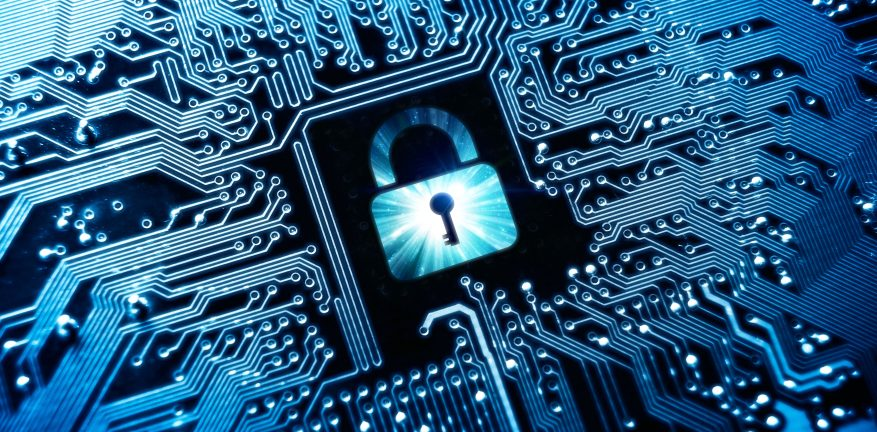
\includegraphics[scale = 0.5]{img.jpg}
        
        
        \vfill
        
       A report compiled for the \\
       Summer of Science 2020
            
       \vspace{0.8cm}
     
       
            
       190050115\\
       IIT Bombay\\
       Mumbai,India\\
            
   \end{center}
\end{titlepage}

\section{Introduction}
Before diving into advanced Cybersecurity, a thorough pre-requisite knowledge of network architecture and protocols used in data transfer is required, which has been completed prior to this midterm report.

\section{Network Models}
To understand the network and how data transfer takes place, various models with layered architecture are used. The two most used models are OSI Model and TCP/IP Model.The OSI model is a generic model that is based upon functionalities of each layer. TCP/IP model is a protocol-oriented standard.The OSI has seven layers while the TCP/IP has four layers.
    \begin{center}
        \begin{tabular}{|c|c|}
            \hline
             \textbf{OSI Model} & \textbf{TCP/IP Model}\\
            \hline
            Application Layer & \\ \cline{1-1}
            Presentation Layer & Application Layer\\ \cline{1-1}
            Session Layer& \\ 
            \hline
            Transport Layer & Transport Layer\\
            \hline
            Network Layer & Internet Layer\\
            \hline
            Data Link Layer  & Network\\ \cline{1-1}
            Physical Layer & Access Layer\\
            \hline
            
        \end{tabular}
    \end{center}
I studied a hybrid version of these models emphasizing more or less equally between the functionality and protocol orientation. All the layers are so designed that they can function independent of what happens in the layers below them.

\subsection{Terminologies}
\begin{itemize}
    \item Clients and Servers : Client initiates a communication and server receives the request and provides the service matching to the request.
    \item Protocols : These are the rules and procedures of data transfer. In each layer different protocols are defined which are followed to communicate. 
    \item Sockets (APIs) : These are software interfaces can be understood as the door to different applications running.
    \item Port Numbers: These are the addresses of the different applications. There are a number of pre-assigned port numbers to frequently run applications, and a set of unused port numbers.
    \item Reliable Data Service : If a protocol provides such a guaranteed data delivery service, it is said to provide reliable data transfer.
    \item Throughput : A measure of the rate at which data is transferred.
\end{itemize}

\subsection{Introduction to Layering}
The top-most layer is the reason for Internet's success. Major applications pertaining to web surfing,instant messaging,file sharing,e-commerce,streaming etc. are used by everyone on a daily basis. The fundamental basis of designing applications is writing programs that run on different end-systems and communicate with each other. The architecture of Application layer can be made on a client-server basis or P2P-basis.\\
Residing between the application and network layers, the transport layer is a central piece of the layered network architecture. It has the critical role of providing communication services directly to the application processes running on different hosts.\\
The network layer is one of the most complex layers in the protocol stack. Forwarding and routing are the functions of the network layer.Forwarding involves the transfer of a packet from an incoming link to an outgoing link within a single router. Routing involves all of a network’s routers, whose collective interactions via routing protocols determine the paths that packets take on their trips from source to destination node.\\
A device running link layer protocol is referred as a node.Nodes include hosts, routers, switches, and WiFi access points. Framing,reliable delivery,link access and error detection and correction are the services provided by link layer. For most of the part the link layer is implemented in the Network Interface Card(NIC).\\
Finally the bottom most layer, the physical layer has more to do with the actual hardware used to transmit the data. It defines the electrical, timing and other interfaces by which bits are sent as signals over channels.

\section{Some Important Protocols}
\subsection{HTTP and Web}
Hyper-Text Transfer Protocol (HTTP), the web’s application-layer protocol.
The webpage has various objects such that HTML files, CSS files,images etc. All these are requested through HTTP.HTTP defines how Web clients request Web pages from Web servers and how servers transfer Web pages to clients.
HTTP uses TCP as its underlying transport protocol.Web browsers implement the client side of HTTP and web servers implement the server side of HTTP.\\
The base HTML file references the other objects in the page with the object's URLs. Each URL has two components, the host name of the server that houses the object and the object’s path name.\\
There are two types connections that can be used by HTTP.In Persistent connection which is default the TCP connection on port 80(the default port for HTTP) is left open for further objects,whereas in Non persistent connection for transfer of each object a new TCP connection has to be made and after the transfer is made the connection is closed. This is a brief overview of what happens after each connection-
\begin{enumerate}
    \item The HTTP client sends the HTTP request to server via it's socket.
    \item The server receives the request and the retrieves the object from the mentioned path and sends it back.
    \item The client receives the message.
\end{enumerate}
\textbf{HTTP message format}\\
A typical HTTP message is of this format-\\
\begin{center}
    \begin{verbatim}
    GET /homepage/190050115.html HTTP/4.1
    Host: www.iitb.ac.in
    Connection: close 
    User-agent: Mozilla/5.0
    Accept-language: en
    \end{verbatim}
\end{center}
The first line mentions the method, the URL which is the path to the required file in server and the version of HTTP.The second line is about the address of the server in the internet.The third line says about the client.The last line is one of the content negotiation field.
\\
A typical HTTP response is of the format-\\
\begin{center}
    \begin{verbatim}
    HTTP/4.1 200 OK
    Connection: close
    Date: Tue, 09 Aug 2011 15:44:04 GMT
    Server: Apache/2.2.3 (CentOS)
    Last-Modified: Tue, 09 Aug 2011 15:11:03 GMT Content-Length: 6821
    Content-Type: text/html
    (data data data data data ...)
    \end{verbatim}
\end{center}
The first line has 200 OK which is one of the status codes that tells about the connection is established or not.There are other status codes like 400 Bad Request,404 Not Found,505 HTTP Version Not Supported ,etc.The server uses the Connection: close header line to tell the client that it is going to close the TCP connection after sending the message.Other lines are not much of importance and are self explanatory.\\
\subsection{FTP}
In a FTP(File Transfer Protocol) session, the user is sitting in front of one host (the client) and wants to transfer files to or from a remote host. In order for the user to access the remote account, the user must provide a user identification and a password. After providing this authorization information, the user can transfer files from the local file system to the remote file system and vice versa.\\
HTTP and FTP are both file transfer protocols but the main difference between them is that FTP uses two parallel TCP connections to transfer a file, a control connection and a data connection.\\
The control connection is used for sending control information between the two hosts—information such as user identification, password, commands to change directories, and commands to “put” and “get” files. The data connection is used to actually send a file.\\
The FTP server keeps a note on the state of the client, that is it keeps a track on what changes the client is making.Thus there is a limitation on the number of sessions that FTP can maintain.\\
There is typically a one-to-one correspondence between the command that the user issues and the FTP command sent across the control connection.Some commands are -
\begin{itemize}
    \item USER username: Used to send the user identification to the server.
    \item PASS password: Used to send the user password to the server.
    \item LIST: Used to ask the server to send back a list of all the files in the current directory.
    \item RETR filename: Used to retrieve a file from the current directory.
    \item STOR filename: Used to store a file into the current directory.
\end{itemize}
As this is one-to-one interaction type protocol each command is followed by one reply.Some replies are-
\begin{itemize}
    \item 331 Username OK, password required
    \item 425 Can’t open data connection
    \item 452 Error writing file
\end{itemize}
\subsection{DNS(Domain name system)}
The DNS is a distributed database implemented in a hierarchy of DNS servers.It is an application-layer protocol that allows hosts to query the distributed database.
DNS is commonly employed by other application layer protocols like HTTP,SMTP,and FTP to translate user supplied hostnames to IP addresses.The working procedure is summarised as follows-
\begin{enumerate}
    \item The client side of the DNS runs on the system itself(in your browsers if you are running an web application).
    \item The using application provides the URL of the server to the DNS client.
    \item The client then sends a query containing the hostname to a DNS server.
    \item The client receives the IP address of the server.
    \item The application that implemented the DNS then uses that IP address to create a transport layer connection.
\end{enumerate}
DNS might appear to be adding a huge delay the connection but the desired IP address is often cached in a “nearby” DNS server, which helps to reduce DNS network traffic as well as the average DNS delay.\\
DNS is implemented as a distributed hierarchical database. There are three classes of DNS servers—root DNS servers, top level domain (TLD) DNS servers, and authoritative DNS servers organized in a hierarchy.
\begin{itemize}
    \item Root DNS servers - These are in the topmost level in hierarchy. In fact each “server” is actually a network of replicated servers, for both security and reliability purposes.
    \item Top-level domain (TLD) servers - These servers are responsible for top-level domains such as com, org, net, edu, and gov, and all of the country top-level domains such as in, uk, fr,and jp.
    \item Authoritative DNS servers- Every organization with publicly accessible hosts (such as Web servers and mail servers) on the Internet must provide publicly accessible DNS records that map the names of those hosts to IP addresses.The organisation can have it's own DNS server or can pay to some DNS service provider.
\end{itemize}
The DNS working can be iterative or recursive.In the iterative way the client first searches it's cache and if the address is not found then it approaches the root server and then root server either returns the address if it is there in it's cache or returns the address of the TLD server that contains the desired address, this is repeated by TLD.\\
In the recursive method the root server upon being asked directly asks the TLD who asks the Authoritative servers,if at any level the address is found then it gets returned in the same way it was asked. It is more like the stack implementation.\\\\
\textbf{DNS Records}\\
The DNS servers that together implement the DNS distributed database store resource records,that provide hostname to IP address mappings.A resource record contains four fields-
\begin{center}
    \begin{verbatim}
        {Name,Value,Type,TTL}
    \end{verbatim}
\end{center}
TTL is the time to live of the resource record,it determines when a resource should be removed from a cache.Name and Value depend on Type.If Type=A, then Name is a hostname and Value is the IP address for the hostname.If Type=NS, then Name is a domain and Value is the host- name of an authoritative DNS server that knows how to obtain the IP addresses for hosts in the domain.There are other Types that are related to other services provided by DNS other than hostname-address matching.\\
\textbf{DNS Messages}
There are two types of DNS messages query and reply.Each message has a specific format which contains the header section(which has a number of fields),Question section,Answer section,Authority section and Additional information section.\\
\subsection{UDP}
It is a transport layer protocol.It is a connection less protocol because it does not check whether a message is received or not,i.e. it does not make any connection with the other side. It does as little as the transport layer is ought to do. Although not reliable it is quite fast.DNS is an example of an application-layer protocol that typically uses UDP.\\\\
\textbf{UDP Segment structure}\\
\begin{figure}
\begin{center}
    
        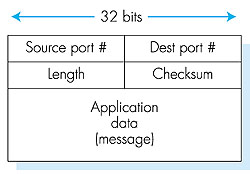
\includegraphics{udp2.jpg}
    \caption{UDP segment}

\end{center}
 \end{figure}
The UDP segment structure is broadly divided into two sections the header section and the data section.The header has only four fields each consisting of two bytes.They are Source port,Destination port,Length and Checksum.The port numbers allow to pass the data to the correct application in the hosts.The length field is the number of bytes in the UDP segment.The checksum helps in error detection.\\
UDP provides error detection at the transport layer, on an end-end basis. This is an example of the implementation of end to end principle in OSI model.
\subsection{TCP}
TCP, the internet transport layer protocol implements reliable data transfer which means it guarantees that all the segments reach the host, that too without any error. TCP is said to be connection-oriented because to send data, the two processes must first “handshake” with each other that is, they must send some preliminary segments to each other to establish the connection. A TCP connection provides a full-duplex service that means two way data transfer occurs between the hosts. TCP is also a point to point service which means it connects a single sender to a single receiver.\\\\
\textbf{Establishing Connection}\\
The connection is established in a three-way handshake process.This happens through these three steps-
\begin{enumerate}
    \item Client sends a TCP segment to the server. A field in the header is marked to differentiate this as a special initiation segment.It is called SYN segment.
    \item After receiving the request the server processes and prepares itself to accept data by allocating variables and buffers. Then the server returns another special segment back to the client to send data.It is called SYNACK segment.
    \item Upon receiving the segment the client also prepares itself to receive data from the upper layer by allocating buffer and variables.The client then re sends another connection granted segment thus confirming the connection.
\end{enumerate}
\begin{figure}
\begin{center}
    
    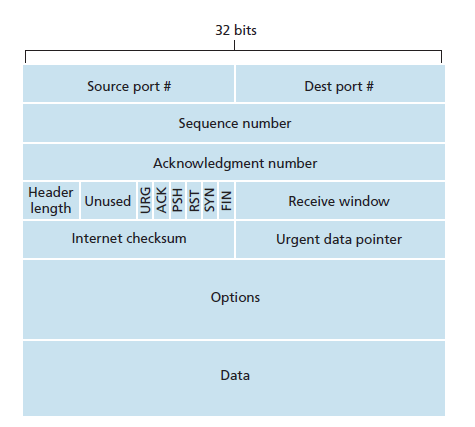
\includegraphics{3.29.png}
    \caption{TCP segment}

\end{center}
 \end{figure}
During the initiation of the connection the sequence numbers are also sent which then plays a vital part during the data transfer.The data transfer during TCP is based on the principle that the segment sent by the client must by ACKed(acknowledged) by the server. If the ACK message is not received by the sender within a particular time period which is decided by a timer which starts after the segment is sent, then the sender re sends the same segment again.Now let us give a brief overview of how data transfer occurs.\\
TCP segments are assigned sequence numbers which helps to maintain reliable transfer as well as helps in ordering the segments when received at the other side.The next side maintains a to be expected sequence number.If the expected sequence number arrives then it sends back an ACK message. It is very possible that the segments may arrive out of order or some segments in between might be lost.To solve this the sender uses duplicate ACKing, which means if a segment which was not yet expected arrives is stored in the buffer and an ACK message of last in-order received message is sent. On the sender side on receiving the ACK message the window frame(which is the collection of segments that have been sent and not ACKed) slides forward.If the sender does not receive the ACK message within a stipulated time then it needs to re-transmit the segment and again start the timer.The estimated round trip time(RTT) for a segment is calculated through a formula-
\[
    EstimatedRTT = (1 – \alpha) \times EstimatedRTT + \alpha \times SampleRTT
\]
where the recommended value of  $\alpha$ is 0.125\\
In addition to estimated RTT we also  have to calculate the variability in RTT which is DevRTT given by
\[
DevRTT = (1 – \beta) \times DevRTT + \beta \times | SampleRTT – EstimatedRTT |
\]
The major advantages of using TCP is that it maintains the \textbf{Flow Control} and \textbf{Congestion Control}. When the senders keeps on accepting more data from the application at a rate which is more than it transfers leading to filing up of the buffer which further leads to data loss.TCP puts a limitation on the amount of data it accepts at a particular time thus ensuring Flow Control.\\
Congestion control is a similar process happening in the receiver side. Flow control and congestion control may seem to be same but yet they have differences as congestion control is network dependent while flow control is not.

\subsection{Internet Protocol}
We are addressing the widespread network layer protocol.The services that this protocol provides is basically forwarding and addressing. The global internet uses this as it's network layer protocol.The segments that have been received from the transport layer gets enclosed in another header to form a datagram(the units formed in the network layer).
\begin{center}
\begin{figure}
    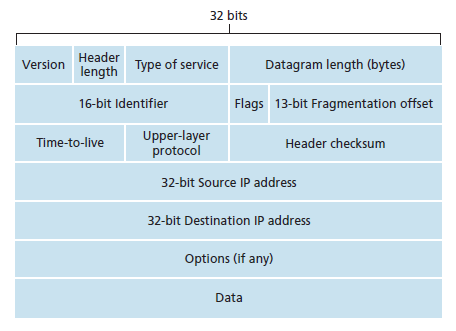
\includegraphics{ip.png}
    \caption{IPv4 datagram}
\end{figure}
\end{center}
\textbf{IP Datagram Fragmentation} is another essential service that is provided. Different routers that the datagrams encounters during it's transmission path have different maximum amount of data that a link layer component can carry, measured in MTU(Maximum Transmission Unit). When the size of data is more than the MTU of the link layer component then data losses will occur. IP solves this problem by allowing breaking the data into smaller fragments and implementing the reforming the datagram from it's fragments upon arriving at the destination.\\
IPv4 is a version of IP that was majorly used in the near past and the main service that IP provides is addressing of the hosts. Lets have a look into the IPv4 addressing.\\
Each IP address is 32 bit long. So there can be $2^{32}$ possible address.These addresses are typically written in a dotted decimal notation, in which each byte of the address is written in its decimal form and is separated by a period (dot) from other bytes in the address. Each interface on every host and router in the global Internet must have an IP address that is globally unique, but they are not named in a random manner rather are determined by the subnet to which they are connected.\\
IP addressing assigns an address to this subnet: for example a.b.c.0/x, where the /x notation, sometimes known as a subnet mask, indicates that the leftmost 24 bits of the 32-bit quantity define the subnet address.The connected interfaces thus can have the addresses a.b.c.1/x,a.b.c.2/x and so on.The Internet’s address assignment strategy is known as Classless Interdomain Routing(CIDR).An organization is typically assigned a block of contiguous addresses, that is, a range of addresses with a common prefix. The IP addresses of devices within the organization will share the common prefix. This is more like having an address for a subnet which further has all the address of the hosts it is composed of. This significantly reduces the forwarding tables, since only maintaining the organization's prefix can help to reach the destination host. \\
\textbf{255.255.255.255} This is the IP address you might have seen a lot of times.This is IP's broadcast address which means when you send something to this IP address the data gets transmitted to all the hosts in the subnet.
\subsubsection{DHCP}
Dynamic Host Configuration Protocol(DHCP) is an essential network layer protocol and operates in synchronization with IP, so we discuss it within IP protocol.This protocol is responsible for automation of the process of address allocation. The DHCP can be configured so that a host gets the same IP address every time it gets connected to internet or can have temporary addresses which are different every session. The user inside the organisation is expected to get connected to different subnets inside(liking you are connecting in library or lecture hall), so a temporary address at each session is more viable. This also minimizes the total number of addresses required as at a time only limited number of hosts are connected. \\Thsese addresses allocation process happens at various dedicated DHCP servers. The host that wants an address broadcasts a message on 255.255.255.255 and then the nearest server then rebroadcasts the reply back. Then the host again sends a request message and the DHCP then ACKs that request.
\subsubsection{IPv4 vs IPv6}
IPv6 is the newer version of Internet Protocol and the main reason it was devised was internet was running out of addresses that the 32 bit IPv4 was providing. The IPv6 which can accommodate 128 bits addresses is expected to be never getting exhausted. Along with that some new fields were introduced,some modified fields were modified and some fields were removed. The main problem that internet has today is to think of how we can transit from IPv4 systems to IPv6 systems at a time. IPv6 was so designed that it can handle IPv4 datagrams but the other way round it does not work. So almost all the systems that are being designed today have both IPv4 and IPv6 compatibility in a vision of complete transition in the future. Various methods such as \textbf{Tunneling} which helps in transmitting data from IPv6 to IPv4 format by appending the changed fields in the data of IPv4 itself and recovering them when it reaches an IPv6 capable system.\\
\subsection{ICMP}
Internet Control Message Protocol is used by hosts and routers to communicate net- work-layer information to each other.The most typical use of ICMP is for error reporting.ICMP is often considered part of IP but architecturally it lies just above IP, as ICMP messages are carried inside IP datagrams.\\
ICMP messages have a type and a code field, and contain the header and the first 8 bytes of the IP datagram that caused the ICMP message to be generated.Some popular ICMP messages are-
\begin{center}
    \begin{tabular}{|c|c|c|}
    \hline
         ICMP Type & Code & Description  \\ \hline
         0  & 0 & echo reply(to ping)\\
         3 & 0 & destination network unreachable\\
         8 & 0 & echo request\\
         11 & 0 & TTL expired\\
    \hline    
    \end{tabular}
\end{center}
ICMP messages can be used to trace routers in the network, they are also used by firewalls and intrusion detecting system to resist against threats.\\
\section{Cryptography}
\subsection{OSI Security Architecture}
\begin{enumerate}
    \item \textbf{Security Attacks}\\
    Compromise of information that was intended not to be shared.
    \item \textbf{Security Mechanism}\\
    The procedures which are adopted to stop information breach.
    \item \textbf{Security Service}\\
    The methods that enhance the security protection and help to prevent and protect against security attacks.
\end{enumerate}
\subsection{Terminologies}
\begin{itemize}
    \item Plain text- This is the message that is intended to be encrypted.
    \item Encryption Algorithm- The rules that are defined to convert the plaintext to ciphertext.
    \item Secret Key-This is the key that is used to encrypt the plain text and is also used to decrypt the cipher text by the receiver.
    \item Ciphered text- This is the encrypted message.
    \item Decryption algorithm- This is the rule that allows the user to obtain the plaintext from the ciphertext often with the help of the key.
\end{itemize}

\section{Symmetric Ciphers}
Symmetric encryption was the only type of encryption that was prevalent before public key encryption. Even now these are widely used (DES and AES ciphers which are widely used today). Symmetric ciphers can be broadly divided into two categories namely Substitution Ciphers and Transposition Ciphers.
\subsection{Substitution Ciphers}
\subsubsection{Caesar Cipher}
    The Caesar cipher involves replacing each letter of the alphabet with the letter standing k places further down the alphabet.k(0<=k<=25) is the key.\\
A general Caesar ciphers algorithm can be given by-\\
\[C = E(k,p) = (p + k)\mod 26\\
p = D(k,C) = (C - k)\mod 26\\
\]
Here C is the ciphertext p is the plain text, k is the key, E and D are encryption and decryption algorithms respectively.\\
This was one the earliest ciphers and can be easily cracked by checking all possible keys and then checking which key results in a sensible plaintext.
\subsubsection{Monoalphabetic Cipher}
This uses a random permutation of english alphabet letters and then maps each letter to an unique letter.Thus this increases the number of keys to 26! thus eliminating the bruteforce crack.
But this can also be cracked by plotting the statistical relative frequency of use of the letters, which will then help to notice the patterns in the cipher text and thus ultimately generating the key.
More powerful techniques if the above still does not help that includes checking for the frequency of the "digrams"(which are commonly used two letter words/pairs) and mapping them to the cipher text can be applied.
This can be further extended to further check for tigrams,polygrams etc.

\subsubsection{Hill Cipher}
This multi-letter linear algebra based cipher is used as follows. At first the letters are mapped to corresponding numbers and then the plaintext is treated as a vector of those numbers. Then a unique matrix is chosen which is then multiplied with the plaintext to obtain the cipher text. The major advantage of using such a cipher is that different plain text characters can get mapped to same cipher text character.
\[
C = E(K,P) = PK\mod 26
\]
\[
P = D(K,C) = CK^{-1}\mod 26 = PKK^{-1} = P
\]
This can also be cracked if we have sufficient number of plaintext and their corresponding ciphertext(which ultimately transforms into a problem of solving linear equations).
\subsubsection{Polyalphabetic Ciphers}
These techniques are based on two techniques, a set of related mono alphabetic substitution rules are used and the key determines which rule is to be used to ciphers the text.
Some of the techniques are:\\
\begin{itemize}
    \item \textbf{Vigenere Cipher}
    The first letter of the key is added to the first letter of the plaintext, mod 26, the second letters are added, and so on through the first m letters of the plaintext. For the next m letters of the plaintext, the key letters are repeated. This process continues until all of the plaintext sequence is encrypted.General equation is
\[
    C_i =(p_i + K_i\mod m)\mod 26
\]
The strength of this cipher is that there are multiple ciphertext letters for each plaintext letter but still all the structure is not lost and some information from the frequency relations can be used to find the plaintext if the key is small then it is easier.There was an improvement to this by making the key longer through an auto key system in which the keyword is concatenated to the plain text to provide a running key.

\item \textbf{Vernam cipher}
The idea was to chose a keyword such that has no statistical relationship with the plaintext.
\\
\begin{figure}
\begin{center}
    
    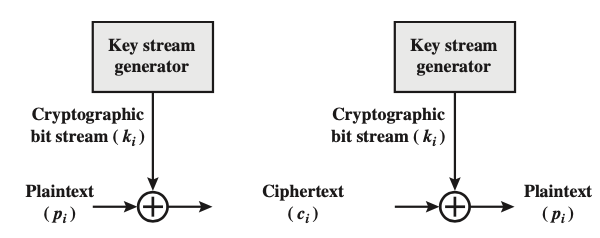
\includegraphics[scale=0.60]{images/vernam.png}
    \caption{Vernam Cipher}

\end{center}
 \end{figure}

\[ c_i = p_i \oplus k_i\text{ where}\\\]
\[p_i = i^{th} \text{ binary digit of plaintext}\\ \]
\[k_i = i^{th} \text{ binary digit of key}\\\]
\[c_i = i^{th}  \text{ binary digit of ciphertext} \\\]
\[
\oplus = \text{XOR operation}\\
\]  
\end{itemize}   
\subsubsection{One Time Pad}
This is the unbreakable algorithm which is based on the idea of using a key as long as the plaintext.The key is completely random and is used only once, so after use the key is discarded. But this method is not that practical because we need constant supply of random characters in large quantities which might be a problem to store and generate. Also for a message we need to transfer a key that is as long as the plaintext so it can be a daunting task to do so.
\subsection{Staganography}
This is completely different method of hiding the message than cryptography but this method has been in use since ages. This method is based on concealing the existence of message itself.
Since earlier days things like character marking, invisible ink, pin punctures etc have been used. Modern use of steganography involves hiding a message by using the least significant bits of frames on a CD.Sometimes both encryption and staganography are used where the message is first encrypted using an algorithm and then hidden.
\subsection{Block Ciphers}
A block cipher is one in which a block of plaintext is treated as a whole and used to produce a ciphertext block of equal length. Typically, a block size of 64 or 128 bits is used. It is an alternative to stream cipher where encryption happens one bit at a time.\\
Suppose we chose blocks of size n, so we have total $2^n$ possible plaintext for the block.We must chose the algorithm such that each block can be mapped to a cipher text just like a bijective function mapping. This can be thought analogous to Hill Cipher technique which used a matrix key to map the plaintext to its ciphertext.This again comes with the defects that were with Hill Cipher technique.This inefficiency of this block cipher design is what proved to be a motivation for Feistel to design his algorithm.
\subsubsection{Feistel Cipher}
This alternates substitution and permutation and is based on the concept of product cipher,which is the execution of two or more simple ciphers in sequence in such a way that the final result or product is cryptographically stronger than any component ciphers.\\
The inputs to the encryption algorithm are a plaintext block of length 2w bits and a key K. The plaintext block is divided into two halves, $L_0$ and $R_0$. The two halves of the plaintext pass through n rounds of processing and then combine to produce the ciphertext block. Each round i has as inputs $L_{i - 1}$ and $R_{i - 1}$ derived from the previous round, as well as a subkey $K_i$ derived from the overall K. In general, the subkeys $K_i$ are different from K and from each other.\\
All rounds have the same structure.A substitution is performed on the left half of the plaintext. This is done by applying a round function F to the right half of the data and then taking the XOR of the output of that function and the left half of the data. The round function has the same general structure for each round and is generated by operations on the subkey $K_i$ on the right half.Following this a permutation is performed that is based on interchanging the two half of the data.\\
\begin{figure}
\begin{center}
    
    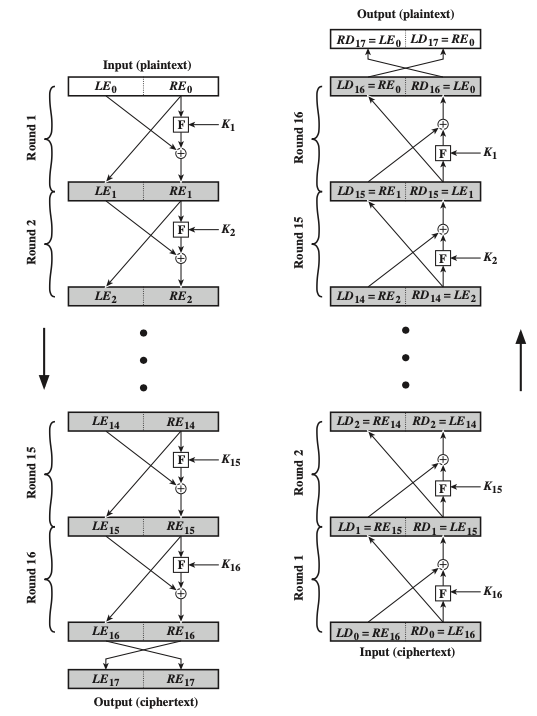
\includegraphics[scale = 0.70]{images/fiestel.png}
    \caption{Fiestel Cipher}

\end{center}
 \end{figure}
Strength of Feistel Cipher is based on Block size, key size, number of rounds, subway generation algorithm, and round function F.\\
Decryption algorithm-\\
This is the exact reverse of the encryption process. The algorithm remains exactly same to the encryption with the input being the ciphertext and the subkeys are fed into the system in the exact reverse order.

\subsection{Data Encryption Standard(DES)}
The algorithm is referred to as DEA(Data Encryption Algorithm). For DEA the data is encrypted within 64 bit blocks using a 56 bit key. With the advancement of computational power, weekend the DES but then double DES and triple DES were started to be used where the DES algorithm was just repeated two and three times. The DES can be represented as follows:
\\
\\
\begin{figure}
\begin{center}
    
    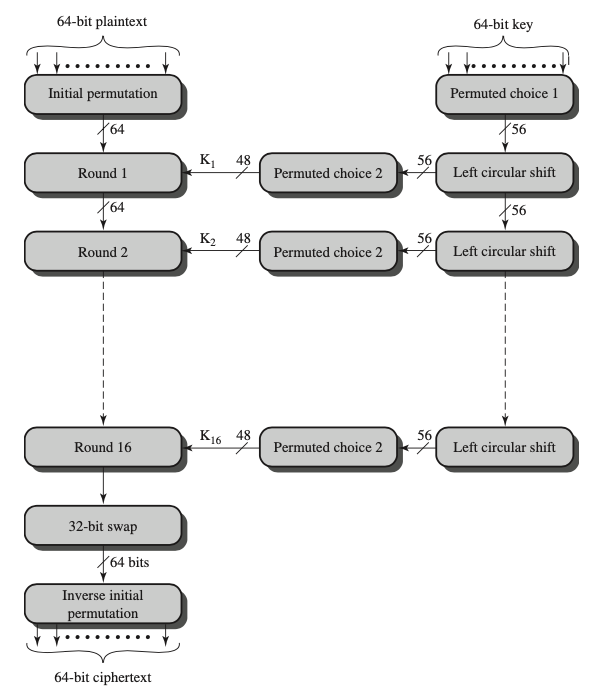
\includegraphics[scale = 0.6]{images/des.png}
    \caption{DES}

\end{center}
 \end{figure}
As with any Feistel cipher, decryption uses the same algorithm as encryption, except that the sequence of the subkeys is reversed. Additionally, the initial and final permutations are reversed.
\textbf{Avalanche Effect} used in DES is a desirable property of an encryption algorithm which refers to that a small change in the plaintext and key would result a significant change in the ciphertext.\\
The DES is particularly strong because it shows strong Avalanche effect.The large strength of DES was due to use of 56 bit keys but when they were overpowered suggestions to use 128 bit keys were given but we have better alternatives like AES and double and triple DES.\\

All Block Cipher Designs are based on the principles of Number of Rounds ,design of the encryption function and the key generation algorithm and the variation in these parameters decide the strength of the cipher.

\subsection{Advanced Encryption Standard(AES)}
In AES, all operations are performed on 8-bit bytes. The arithmetic operations of addition, multiplication, and division are performed over the finite field Galois Field($2^8$).A Galois field is a set in which we can do addition, subtraction, multiplication, and division which are covered under certain rules.\\
The below image shows the overall structure of the AES encryption process. The cipher takes a plaintext block size of 128 bits, or 16 bytes. The key length can be 16, 24, or 32 bytes (128, 192, or 256 bits).\\
\\
\begin{figure}
\begin{center}
    
    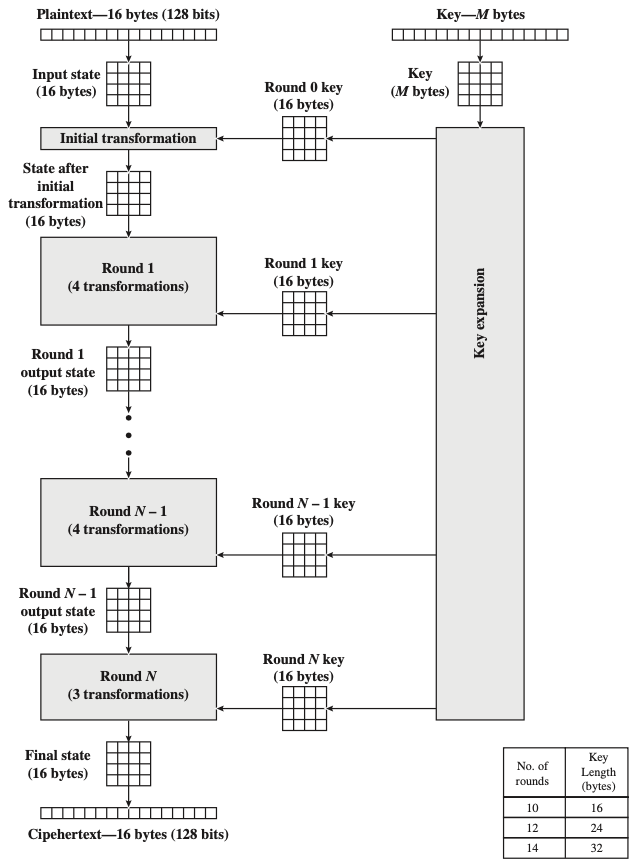
\includegraphics[scale = 0.60]{images/AES.png}
    \caption{AES}

\end{center}
 \end{figure}
The input to this encryption algorithm is a $4\times4$ square matrix of bytes. The block is copied into the state array which is modified in each of the rounds of encryption or decryption and then at the final stage the stage array is copied into the output matrix.\\
During each round four different stages are used :
\begin{itemize}
    \item Substitute Bytes :\\
    It is based on a simple table lookup. AES defines a $16\times16$ matrix of byte values, called an S-box, that contains a permutation of all possible 256 8-bit values. Each individual byte of State is mapped into a new byte with the help of S-box.
    \item Shift Rows : \\
    This happens in the following manner. The first row is not altered. The second row is shifted circularly by 1 byte at a time. The third row is shifted circularly 2 byte at a time and the fourth row by 3 bytes at a time.
    \item Mix Columns : \\
    This operation operates on each column individually.Each byte of a column is mapped into a new value that is a function of all four bytes in that column. The transformation can be defined by a matrix multiplication on state matrix.
    \item Add Round Key :\\
    For both encryption and decryption, the cipher begins with an AddRoundKey stage, followed by nine rounds that each includes all four stages, followed by a tenth round of three stages.In this stage the 128 bit state matrix is XOR-ed with 128 bit round key.The inverse add round key transformation is identical to the forward add round key transformation, because the XOR operation is its own inverse.
\end{itemize}
Only the Add Round Key requires the key, the other stages do not require the knowledge of any key. Thus the AddRoundKey stage is responsible for securing and the other stages are responsible for adding confusion and diffusion to the matrix. Except the round key stage others are reversible even without the knowledge of the key.\\
AES is an advanced algorithm and is yet to be broken.
\subsection{Multiple Encryption}
This refers to the extended algorithms of DES where DES is performed multiple times (usually 2 times for double DES and 3 times for triple DES) to increase the security to unbreakable standards.\\
Double DES has two encryption stages and two keys.Given a plaintext P and two encryption keys K1 and K2, ciphertext C is generated as \\
C = E(K2, E(K1, P))\\
Decryption requires that the keys be applied in reverse order,\\
P = D(K1, D(K2, C))\\
Double DES works because it is not reducible to single DES, i.e. every time there cannot exist a key K3 for a given K1,K2 such that K3 applied as single DES will perform the encryption done by K2,K2 during double DES.\\
Similarly the triple DES might first appear to use 3 keys, but it has the drawback of requiring a key length of 56$\times$3 = 168 bits, which may be somewhat unwieldy.So as an alternative a triple DES technique with two keys is used.The algorithm can be represented as follows -\\
C = E(K1, D(K2, E(K1, P))) \\
P = D(K1, E(K2, D(K1, C)))\\
The plaintext which are longer than the length of the blocks have to be broken down into blocks of the size of the block cipher. But all those blocks cannot be encrypted using the same key. To apply block ciphering in various situations many modes of operation have been devised.\\
\begin{itemize}
    \item Electronic Codebook :\\
    Each block of plaintext bits is encoded independently using the same key.
    \item Cipher Block Chaining (CBC) :\\
    The input to the encryption algorithm is the XOR of the next block of plaintext and the preceding block of ciphertext.
    \item Cipher Feedback (CFB) :\\
    Input is processed s bits at a time. Preceding ciphertext is used as input to the encryption algorithm to produce pseudo-random output, which is XOR-ed with plaintext to produce next unit of ciphertext.
    \item Output Feedback (OFB) :\\
    Similar to CFB, except that the input to the encryption algorithm is the preceding encryption output, and full blocks are used.
    \item Counter (CTR) :\\
    Each block of plaintext is XOR ed with an encrypted counter. The counter is incremented for each subsequent block.
\end{itemize}

\subsection{Pseudo-random Number Generators(PRNGs)}
Random numbers are frequently used in cryptography. The random numbers must have the property that they are uniformly distributed and they are independent of each other.
Pseudo-random numbers are not truly random numbers rather they are produced by effective  deterministic algorithms but then also they pass most of the tests of random numbers.\\
Pseudo-random numbers generation is initiated by taking a seed as input, this seed is a fixed value. Quite often this seed is generated by true random number generators(for example sound intensities from a running river etc.)
This seed is fed into an algorithm which then produces an output. That output is again fed into the algorithm and the resulting output is placed adjacent to initial output or merged in some other way, this cycle continues until a sufficiency long enough random number is generated.

\section{Asymmetric Ciphers}
\subsection{Public-Key Cryptosystems}
Symmetric cryptography had this problem that the key had to be shared secretly. But this is not practical and a perfectly secure method to take a key from one place to another place could not be devised. So a better system that is used today was devised. This system was called the public key crypto systems.\\
It was based on the idea to use two keys between the sender and the receiver. The two keys and the algorithm of encryption was so devised that to encrypt a message you needed one of the keys and to decrypt the message you need the other key.One of these keys was declared as the public key and the other key was called the private key. The public key had to be shared with everyone and the person receiving the message must have the public key to decrypt the message. \\
The system was an extremely clever design and is based as follows. The sender first encrypts the message with the public key of the receiver and then he encrypts with his own private key. As the message was encrypted with the public key of the receiver, only the receiver who has the corresponding private key could decrypt the message. Then the receiver will use the public key of the sender to decrypt the message thus establishing the legitimacy of the sender as well.\\
Other methods also can be used such as Digital Signatures.The sender “signs” a message with its private key. Signing is achieved by a cryptographic algorithm applied to the message or to a small block of data that is a function of the message.\\
Public-Key Cryptosystems can also happen through key exchanges.Two sides cooperate to exchange a session key. Several different approaches are possible, involving the private key(s) of one or both parties.

\subsection{RSA Algorithm}
The idea of public key encryption led to the search of mathematical functions and algorithms that were strong and utilised the two way key sharing technique.One of such successful algorithm is the RSA algorithm devised by Ron Rivest, Adi Shamir, and Len Adleman.\\
RSA makes use of an expression with exponentials. Plaintext is encrypted in blocks, with each block having a binary value less than some number n. Encryption and decryption of the algorithm is based on the following algorithm:\\\\
$C = M^e \mod n$\\
$M = C^d \mod n = (M^e)^d \mod n= M^{ed} \mod n$\\\\
Both sender and receiver must know the value of n. The sender knows the value of e, and only the receiver knows the value of d. Thus, this is a public key encryption algorithm with a public key of PU = \{e, n\} and a private key of PR = \{d, n\}.\\
The relationship between e and d can be expressed as \\\\
$ ed \mod$ $\phi(n)$ = 1 or $e$ and $d$ are multiplicative inverses modulo $\phi(n)$\\\\
Now the question arises how to generate the number n.The scheme is as follows :\\
$p, q$ two prime numbers .......(private, chosen)\\
$n = pq$				............(public, calculated)\\
$e$, with gcd$(\phi(n), e) = 1; 1 < e < \phi(n)$ ..........(public, chosen)\\
$d$ congruent to $e^{-1}$ (mod $\phi(n)$)	..........(private, calculated)\\
Here $\phi$ is the Euler Totient Function.\\
The strength of the algorithm lies in the fact that $\phi(n)$ can be easily calculated if $n = pq $, because \\
$\phi(n) = \phi(p)\times\phi(q)$\\
$\phi(x)$ (if $x$ is prime) = $x-1$\\
The primes are chosen sufficiently large so that it becomes computationally impractical to prime factorise n and determine p, q by the intruder. A typical n has around 200 to 250 digits.
\\
\begin{figure}
\begin{center}
    
    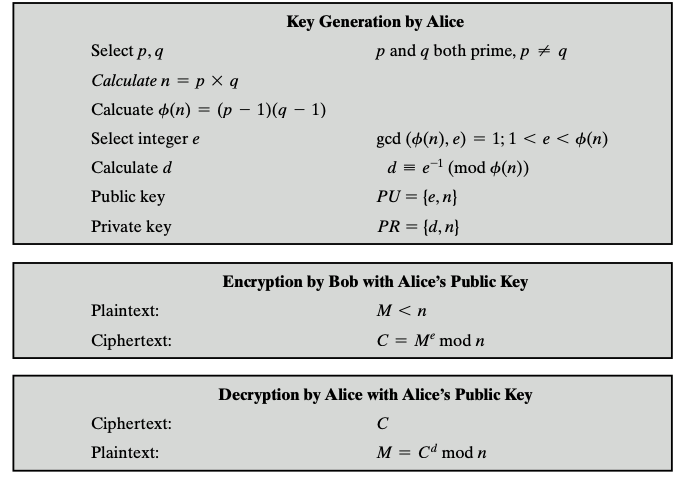
\includegraphics[scale = 0.5]{images/RSA.png}
    \caption{RSA}

\end{center}
 \end{figure}
The RSA system is the most widely used encryption standard used in web and other applications in today's world.It is also the most widely studied public key encryption algorithm. Some other public key encryption algorithms are also there like Diffie Hellman key exchange,Elgamal Cryptographic Systems,Elliptic Curve Arithmetic etc.

\section{Cryptographic Data Integrity Algorithms}

\subsection{Cryptographic Hash Functions}
A hash function H accepts a variable length block of data M as input and produces a fixed size hash value $h = H(M)$.The kind of hash function needed for security applications is referred to as a cryptographic hash function. In other words, the hash function is used as a compressed smaller size representation of the original message. Using only the hash function we cannot derive the message M but this hash code can act as an identity of the message M.\\
The applications of cryptographic hash functions include message authentication, digital signatures, one-way password file, intrusion detection, virus detection, PRNG etc.\\
The requirements of a hash function are :
\begin{itemize}
    \item Function should accept variable input size and fixed output size.
    \item The function should be algorithmically fast enough and efficient.
    \item The function should be preimage resistant (one-way property). That means for any given hash value h, it should be computationally infeasible to find y such that H(y) = h.
    \item The function should be strongly Collision resistant.It should be computationally infeasible to find any pair (x, y) such that H(x) = H(y).
    \item The function should have pseudo-randomness. That means the output of H should meet the standard tests for pseudo-randomness and must show avalanche effect.
\end{itemize}

\subsection{Secure Hash Algorithm(SHA)}
This is the most widely used hash function. After weakening of the initial version,SHA-0 , further versions like SHA-1 were developed.
SHA-1 produces a hash value of 160 bits.Stronger versions of SHA, with hash value lengths of 256, 384, and 512 bits, known as SHA-256, SHA-384, and SHA-512, respectively were devised later on.\\
\textbf{Working of SHA-512}\\
The algorithm takes as input a message with a maximum length of less than $2^128$ bits and produces as output a 512-bit message digest. The input is processed in 1024-bit blocks.The algorithm has been devised as follows-\\
\begin{enumerate}
    \item Append padding bits :\\
    The message is padded so that its length is congruent to 896 modulo 1024.Padding is always added, even if the message is already of the desired length.The padding consists of a single 1 bit followed by the necessary number of 0 bits.
    \\
    \begin{figure}
\begin{center}
    
    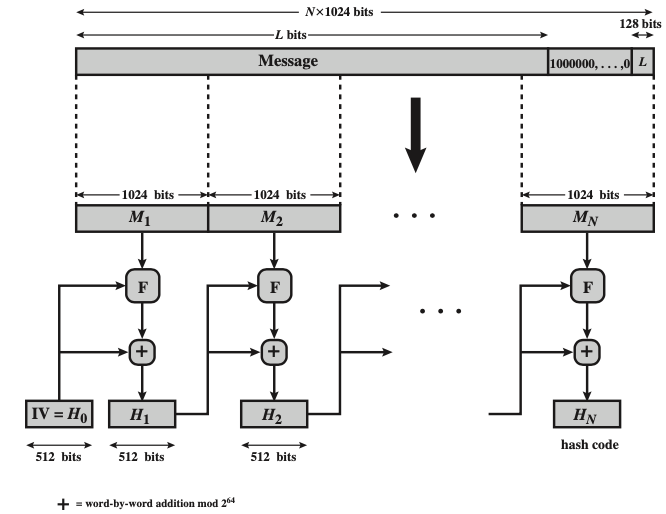
\includegraphics[scale = 0.5]{images/sha.png}
    \caption{SHA}

\end{center}
 \end{figure}
    \item Append length :\\
    A block of 128 bits is appended to the message. This block is treated as an unsigned 128-bit integer and contains the length of the original message.
    Thus the result of appending makes the message 1024 bits long.
    \item Initializing the hash buffer :\\
    A 512 bit buffer, which can be represented as eight 64 bit registers named as a,b,c,d,e and f,are first initialised to a value.This buffer is then modified and the final output is the final state of the buffer.
    \item Process message in 1024-bit (128-word) blocks :\\
    A module consists of 80 rounds, another module repeats after the completion of one module until the full message is covered.Each round takes as input the 512-bit buffer value, abcdefgh, and updates the contents of the buffer. Each round t makes use of a 64-bit value Wt, derived from the current 1024-bit block being processed message.This complicated compression function happens 80 times in each module.
    \item Output :\\
    After all N 1024-bit blocks have been processed, the output from the Nth stage is the 512-bit hash message.
\end{enumerate}

\subsection{Message Authentication}
Message authentication assures that data received are exactly as sent and the sender is legitimate. The hash value of the message sent by the sender is first calculated using the hash algorithm, then the sender sends the message and the hash value to the receiver who on it's end again calculates the hash value of the message and checks whether the message is intact or not. But the hash function must be transported in a secured fashion because if the intruder is able to modify the hash value in between the communication, then the message authentication system fails.\\
Message authentication is achieved using a message authentication code (MAC), also known as a keyed hash function. Typically, MACs are used between two parties that share a secret key to authenticate information exchanged between those parties. The intruder who tries to modify the hash function cannot do without knowing the secret key.\\
\subsection{Digital Signatures}
The operation of the digital signature is similar to that of the MAC. In the case of the digital signature, the hash value of a message is encrypted with a user’s private key. Anyone who knows the user’s public key can verify the integrity of the message that is associated with the digital signature.In this case, an attacker who wishes to alter the message would need to know the user’s private key. These digital signatures can be used for message authentication and now a days are also used in cryptocurrency.\\

\begin{thebibliography}{9}
\bibitem{latexcompanion} 
Jim Kurose,Keith Ross 
\textit{Computer Networking: A Top-Down Approach}.
Addison-Wesley, Pearson.

\bibitem{einstein} 
Tanenbaum, Andrew S. 
\textit{Computer Networks}.
Pretince Hall,Pearson.

\bibitem{Pearson}
William Stallings
\textit{Cryptography and Network Security: Principles and Practice, Sixth Edition}.
Pearson Education Inc.
\end{thebibliography}
\end{document}
